\section{PG Encoding}

Automated design of general purpose processing cores, application-specific
instruction-set processors (ASIPs), and distributed Systems-on-Chip
(SoCs) has gained a lot of attention from academia and industry~\cite{2006_dutt_chapter}.
New formalisms for data-path modelling are proposed~\cite{2010_mokhov_ieee}\cite{2008_sokolov_sdfs},
hardware/software co-design methodology~\cite{1993_alomary_edac}
is actively developed and applied for ASIP performance improvement,
more specific techniques (such as compiler-directed instruction set
optimisation~\cite{2002_qin_date}) are constantly introduced into
the instruction set architecture (ISA) design domain.

\begin{figure}
\begin{centering}
\vspace{-3mm}
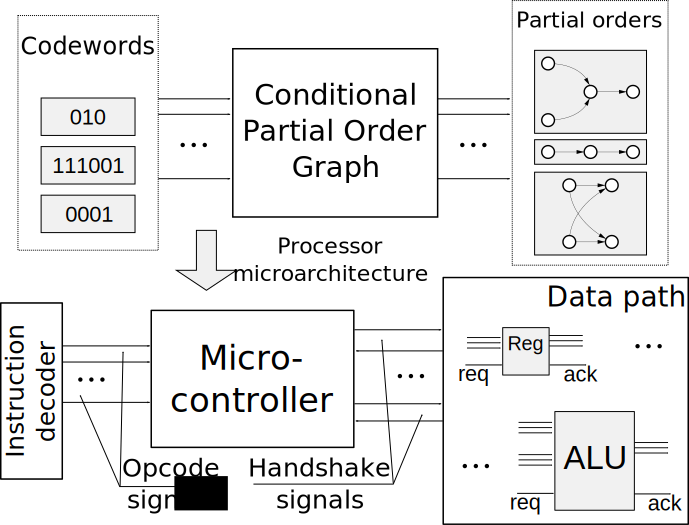
\includegraphics[width=0.6\columnwidth]{fig/control}\vspace{-1mm}

\par\end{centering}

\caption{CPOGs and processor microcontrol\label{fig:Dynamically-reconfigurable-controller}}
\vspace{-3mm}
\end{figure}

{\huge{
TODO: vyzhimka
\begin{itemize}
\item larger set of possible solutions
\item synthesis of optimal decoder
\item SAT
\end{itemize}
}}

Synthesis of instruction sets is a particularly active research area.
There are methods for automated ISA synthesis for a target platform
(according to available system resources and data-path components)
and for given software requirements (e.g. aimed to ease compilation
or reduce program length). These methods eventually produce a structured
set of instructions satisfying certain properties (orthogonality,
completeness, regularity, etc.); instructions are grouped into classes
and each class is allocated a certain opcode interval within the total
code space~\cite{2003_nohl_dac}. At this point automation is typically
stopped or becomes trivial: the instructions are given arbitrary codes
within the allocated intervals. This limits performance due to instruction
decoder circuitry overheads. The problem is usually approached by
ad-hoc heuristics or application-specific optimisation techniques
(see, for example,~\cite{2002_lee_iccad}).

In this chapter we try to solve the general problem of optimal encoding
of a given set of instructions with the aid of the Conditional Partial
Order Graph (CPOG) model introduced recently~\cite{2009_mokhov_phd}\cite{2010_mokhov_ieee}.
The key features of the model are: ability to describe systems in
a compact functional form, and structural synthesis methods which
significantly improve performance of the whole design flow. These
features make the model very efficient for representation and management
of processor instruction sets in hardware and EDA software. A CPOG
is a superposition of a set of partial orders which can be extracted
from it by providing the corresponding codewords, see Figure~\ref{fig:Dynamically-reconfigurable-controller}
(top). It can be regarded as a custom associative memory for storing
cause and effect relations within a predefined set of events.

There are different kinds of systems which can be described with the
model. For example, a processor microcontroller executes partial orders
(or \emph{instructions}) of primitive computational steps (or \emph{microinstructions})
defined on a set of data path operational units, see Figure~\ref{fig:Dynamically-reconfigurable-controller}
(bottom). The order is determined by an \emph{instruction code} --- 
a combination of logical conditions presented
to the controller by the environment~\cite{1994_de_micheli_book}.
To this end, the microcontroller can be seen as an entity which communicates
with two parts of the environment: one part is the source of condition
signals (an instruction decoder) and the other part is a set of controlled
objects with request-acknowledgement interface (data path operational
units which execute the microinstructions).

There are many criteria which determine the choice of a particular
processor architecture and influence design of an instruction set:
functionality, operation modes, resources, etc. In Section~\ref{sec-processor}
we study an example of an instruction set (a subset of MSP430
processor~\cite{mspmanual}) implemented on a minimalistic hardware
platform. However, the main focus of this paper is optimal encoding
of processor instruction sets in the general architecture-independent
context. See~\cite{2011_mokhov_tr} for investigation of the architecture-level
reasoning using the CPOG model.

